\section{Spazio di Lebesgue}

\begin{definition}
    Lo \textbf{Spazio di Lebesgue} è definito come:
    
    $$
        L^1(\mathbb{R}) = \left \{ f: \mathbb{R} \rightarrow \mathbb{R} : \int_\mathbb{R} |f(t)| \ dt < +\infty \right \}
    $$
\end{definition}

Ci riferiamo anche a questo spazio come
\begin{center}
    \textit{L'insieme di tutte le funzioni sempre o assolutamente integrabili in
        modulo}.
\end{center}

\textbf{N.B.} Con la notazione "$< +\infty$" si intende "\textit{è finito}".

\begin{definition}
    Definiamo lo spazio delle funzioni sempre o assolutamente integrabili in
    modulo alla potenza $p$ come:
    
    $$
        L^p(\mathbb{R}) = \left \{ f: \mathbb{R} \rightarrow \mathbb{R} : \int_\mathbb{R} |f(t)|^p \ dt < +\infty \right \}
    $$
    
    $L^p (\mathbb{R})$ è anche detto \textbf{Spazio di Lebesgue al variare di p}
    (con $p \ge 1$).
\end{definition}

\begin{definition}
    Definiamo la \textbf{norma di $L^p$} come:
    
    $$
        ||f||_p = \left( \int_{\mathbb{R}} |f(t)|^p \ dt \right)^{\frac{1}{p}}
    $$
\end{definition}

Prendiamo ora la seguente funzione:

$$
    f : \left] 0, 1 \right] \rightarrow \mathbb{R}, \ \ f(x) = \frac{1}{\sqrt{x}}
$$

e proviamo a vedere se questa sta nello spazio $L^1(\left] 0, 1 \right])$.
\begin{equation}
    \begin{aligned}
        \int_{0}^{1} |\frac{1}{\sqrt{x}}| \ dx & = \int_{0}^{1} \frac{1}{\sqrt{x}} \ dx = \lim_{x \rightarrow 0^+} \int_{x}^{1} \frac{1}{\sqrt{t}} \ dt =          \\
                                               & = \lim_{x \rightarrow 0^+} \int_{x}^{1} t^{-\frac{1}{2}} \ dt = \lim_{x \rightarrow 0^+} [ 2 \sqrt{t} ]_{x}^{1} = \\
                                               & = \lim_{x \rightarrow 0^+} 2 [1 - \sqrt{x}] = 2 < +\infty.
    \end{aligned}
\end{equation}

Concludiamo quindi che $f(x) = \frac{1}{\sqrt{x}} \in L^1(]0, 1])$.

\paragraph{Note:}
\begin{itemize}
    \item $\int_{0}^{1} |\frac{1}{\sqrt{x}}| \ dx = \int_{0}^{1}
              \frac{1}{\sqrt{x}} \ dx$: il modulo scompare perchè
          $\frac{1}{\sqrt{x}}$ nell'intervallo $]0, 1]$ sarà sempre positivo
          !
          
          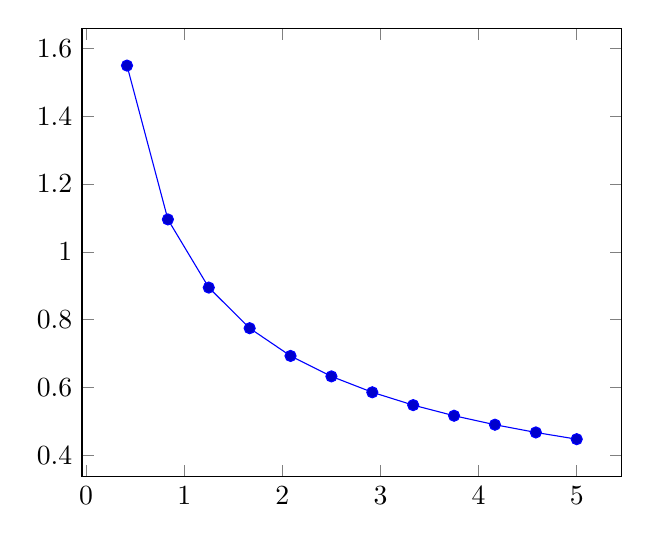
\begin{tikzpicture}
              \begin{axis}%[
                  %       xlabel=$x$, ylabel={$y$}
                  %   ]
                  \addplot {1/sqrt(x)};
              \end{axis}
          \end{tikzpicture}
\end{itemize}

\vspace{1cm}

Ora ci chiediamo se il prodotto di due funzioni che appartengono a $L^1$ sta
ancora in $L^1$. Prendiamo dunque:

$$
    f(x) \cdot f(x) = \frac{1}{x}
$$

e verifichiamo se $\frac{1}{x} \in L^1(]0, 1])$:

\begin{equation}
    \begin{aligned}
        \int_{0}^{1} \frac{1}{x} \ dx & = \lim_{x \rightarrow 0^+} \int_{x}^{1} \frac{1}{t} \ dt = \lim_{x \rightarrow 0^+} [log |t|]_{x}^{1} = \\
                                      & = \lim_{x \rightarrow 0^+} [log 1 - log|x|] = +\infty.
    \end{aligned}
\end{equation}

Deduciamo quindi che non sempre il prodotto di due funzioni che stanno in $L^1$
appartiene a $L^1$.

\paragraph{Note:}
\begin{itemize}
    \item Ricordiamo che $log 1 = 0$
    \item Ricordiamo che $log |x|$ con $x$ che tende a $0^+$ (tende a 0 dalla
          destra) va a $-\infty$
          
          \begin{tikzpicture}
              \begin{axis}%[
                  %       xlabel=$x$, ylabel={$y$}
                  %   ]
                  \addplot {ln(x)};
              \end{axis}
          \end{tikzpicture}
    \item $\lim_{x \rightarrow 0^+} [log 1 - log|x|] = 0 - (-\infty) = +\infty$
\end{itemize}

\vspace{1cm}

Per far sì che il prodotto appartenga a $L^1$ dobbiamo introdurre il concetto di
\textit{\textbf{Prodotto di Convoluzione}}.

\section{Prodotto di Convoluzione}
Il \textbf{Prodotto di Convoluzione} è importante perchè ci permette di
mantenere l'appartenenza allo spazio della singola immagine. Questo, può essere
espresso, in modo formale, nel seguente modo:
\begin{center}
    La \textit{Convoluzione} è una tecnica che consente di regolarizzare le
    funzioni e di approssimarle in $L^p$.
\end{center}

\begin{definition}
    Siano $f \in L^1(\mathbb{R})$ e $g \in L^p(\mathbb{R})$ con $1 \leq p \leq
        +\infty$. \'E possibile definire il prodotto di convoluzione tra $f$ e
    $g$ come:
    
    $$
        \left( f \star g\right)(x) = \int_{\mathbb{R}} f(x - y) g(y) \ dy
    $$
    
    e
    
    $$
        ||f \star g||_p \leq ||f||_1 \cdot ||g||_p.
    $$
    
    Ovvero, il Prodotto di Convoluzione sta in $L^p (\mathbb{R})$
    
    $$f \star g \in L^p(\mathbb{R})
    $$
    
    Risulta quindi vero che $||f \star g||_p < +\infty$.
    
\end{definition}

\vspace{0.3cm}

\textbf{N.B.} Il Prodotto di Convoluzione eredita le migliori proprietà delle due
funzioni.

\vspace{1cm}

Diamo ora il seguente lemma riassuntivo che raccoglie tutte le principali
proprietà del prodotto di convoluzione.

\begin{lemma}
    Date $f, g, h \in L^1(\mathbb{R})$, risulta:
    
    \begin{enumerate}
        \item $f \star g = g \star f$ (proprietà commutativa);
        \item $f \star (g + h) = (f \star g) + (f \star h)$ (proprietà
              distributiva rispetto alla somma);
        \item $(f \star g) \star h = f \star (g \star h)$ (proprietà
              associativa);
        \item posto $\tau_a f(x) := f(x + a), \ x \in \mathbb{R}$ (operatore di
              traslazione,) risulta:
              $$
                  \tau_a (f \star g) = (\tau_a f) \star g
              $$
              (invarianza per traslazioni).
    \end{enumerate}
\end{lemma}

